\subsection{Experimental setup}
\label{sec:setup}

\subsubsection{System}
\label{sec:system}

\ignore{In our experiments, }We employ a server equipped with an x86-based 64-core AMD EPYC-7742 processor. It operates at a clock frequency of $2.25$ GHz and is paired with $512$ GB of DDR4 system memory. Each core features a $4$ MB L1 cache, a $32$ MB L2 cache, and a shared L3 cache of $256$ MB. The server runs on Ubuntu 20.04.


\subsubsection{Configuration}
\label{sec:configuration}

\begin{table}[hbtp]
  \centering
  \caption{List of $12$ graphs retrieved from the SuiteSparse Matrix Collection \cite{suite19} (with directed graphs indicated by $*$). Here, $|V|$ denotes the number of vertices, $|E|$ denotes the number of edges (after making the graph undirected by adding reverse edges), and $|\Gamma|$ denotes the number of communities obtained with \textit{Static Leiden} algorithm \cite{sahu2023gveleiden}.}
  \label{tab:dataset-large}
  \begin{tabular}{|c||c|c|c|}
    \toprule
    \textbf{Graph} &
    \textbf{\textbf{$|V|$}} &
    \textbf{\textbf{$|E|$}} &
    \textbf{\textbf{$|\Gamma|$}} \\
    \midrule
    \multicolumn{4}{|c|}{\textbf{Web Graphs (LAW)}} \\ \hline
    indochina-2004$^*$ & 7.41M & 341M & 2.68K \\ \hline
    arabic-2005$^*$ & 22.7M & 1.21B & 2.92K \\ \hline
    uk-2005$^*$ & 39.5M & 1.73B & 18.2K \\ \hline
    webbase-2001$^*$ & 118M & 1.89B & 2.94M \\ \hline
    it-2004$^*$ & 41.3M & 2.19B & 4.05K \\ \hline
    sk-2005$^*$ & 50.6M & 3.80B & 2.67K \\ \hline
    \multicolumn{4}{|c|}{\textbf{Social Networks (SNAP)}} \\ \hline
    com-LiveJournal & 4.00M & 69.4M & 3.09K \\ \hline
    com-Orkut & 3.07M & 234M & 36 \\ \hline
    \multicolumn{4}{|c|}{\textbf{Road Networks (DIMACS10)}} \\ \hline
    asia\_osm & 12.0M & 25.4M & 2.70K \\ \hline
    europe\_osm & 50.9M & 108M & 6.13K \\ \hline
    \multicolumn{4}{|c|}{\textbf{Protein k-mer Graphs (GenBank)}} \\ \hline
    kmer\_A2a & 171M & 361M & 21.1K \\ \hline
    kmer\_V1r & 214M & 465M & 10.5K \\ \hline
  \bottomrule
  \end{tabular}
\end{table}

\begin{table}[hbtp]
  \centering
  \caption{List of $5$ real-world dynamic graphs\ignore{, i.e., temporal networks}, sourced from the Stanford Large Network Dataset Collection \cite{snapnets}. Here, $|V|$ denotes the number of vertices, $|E_T|$ represents the count of temporal edges (inclusive of duplicates), and $|E|$ indicates the number of static edges (without duplicates).}
  \label{tab:dataset}
  \begin{tabular}{|c||c|c|c|c|}
    \toprule
    \textbf{Graph} &
    \textbf{\textbf{$|V|$}} &
    \textbf{\textbf{$|E_T|$}} &
    \textbf{\textbf{$|E|$}} \\
    \midrule
    sx-mathoverflow & 24.8K & 507K & 240K \\ \hline
    sx-askubuntu & 159K & 964K & 597K \\ \hline
    sx-superuser & 194K & 1.44M & 925K \\ \hline
    wiki-talk-temporal & 1.14M & 7.83M & 3.31M \\ \hline
    sx-stackoverflow & 2.60M & 63.4M & 36.2M \\ \hline
  \bottomrule
  \end{tabular}
\end{table}


We utilize 32-bit unsigned integers for vertex IDs and 32-bit floating-point for edge weights. For computation involving floating-point aggregation, like total edge weights and modularity, we switch to 64-bit floating-point. Affected vertices and changed communities are represented by 8-bit integer vectors. During the local-moving, refinement, and aggregation phases, we employ OpenMP's dynamic scheduling with a chunk size of $2048$ for load balancing. However, for the aggregation phase in Naive-dynamic (ND), Delta-screening (DS), and Dynamic Frontier (DF) Leiden, a chunk size of $32$ is used. We utilize state-of-the-art parallel Leiden \cite{sahu2024fast}, incorporating our ND, DS, and DF Leiden atop it. For real-world dynamic graphs (discussed in Section \ref{sec:performance-comparison-temporal}), which aggregate slowly, we disable aggregation tolerance - setting it to $1$. This ensures all desirable community aggregations occur, yielding higher modularity scores compared to the default of $0.8$. For consistency, we apply this to static Leiden as well - to avoid comparing apples-to-oranges. We run all\ignore{parallel} implementations on $64$ threads and compile using GCC 9.4 with OpenMP 5.0.
% Key parameters include an iteration tolerance $\tau$ of $10^{-2}$ for the local-moving phase, a \textit{TOLERANCE\_DECLINE\_FACTOR} of $10$ for threshold scaling optimization \cite{lu2015parallel}, a \textit{MAX\_ITERATIONS} of $20$ for the local-moving phase per pass, and a \textit{MAX\_PASSES} of $10$ \cite{sahu2024fast}.

\subsubsection{Dataset}
\label{sec:dataset}

We conduct experiments on $12$ large real-world graphs with random batch updates, listed in Table \ref{tab:dataset-large}, obtained from the SuiteSparse Matrix Collection. These graphs have between $3.07$ million and $214$ million vertices, and $25.4$ million to $3.80$ billion edges. For experiments involving real-world dynamic graphs, we utilize five temporal networks sourced from the Stanford Large Network Dataset Collection \cite{snapnets}, detailed in Table \ref{tab:dataset}. Here, the number of vertices span from $24.8$ thousand to $2.60$ million, temporal edges from $507$ thousand to $63.4$ million, and static edges from $240$ thousand to $36.2$ million. However, we would like to note that existing temporal graphs in the SNAP repository \cite{snapnets} are mostly small\ignore{(with one exception)}, limiting their utility for studying our proposed parallel algorithms. With each graph, we ensure that all edges are undirected and weighted, with a default weight of $1$. Since most publicly available real-world weighted graphs are small in size, we do not use them here --- although our parallel algorithms can handle weighted graphs without any modification.

We also do not use SNAP datasets with ground-truth communities, as they are non-disjoint, while our work focuses on disjoint communities. Nevertheless, we wish to note that the goal of community detection is not necessarily to match the ground truth, as this may reflect a different aspect of network structure or be unrelated to the actual structure, and focusing solely on this correlation risks overlooking other meaningful community structures \cite{peel2017ground}.


\subsubsection{Batch generation}
\label{sec:batch-generation}

We take each base graph from Table \ref{tab:dataset-large} and generate random batch updates \cite{com-zarayeneh21}, comprising an $80\% : 20\%$ mix of edge insertions and deletions to emulate realistic batch updates, with each edge having a weight of $1$. Batch updates are generated with unit-weighted edges for simplicity, without affecting results, as the algorithms handle arbitrary edge weights.\ignore{In the batch updates, $??\%$ edge deletions are intra-community, while $??\%$ insertions are cross-community, reflecting strong connectivity of identified communities.} Since the random batch updates are processed separately, the graph does not converge toward a random structure. This enables testing on diverse graph classes. All updates are undirected; for every edge insertion $(i, j, w)$, we also include $(j, i, w)$. To prepare the set of edges for insertion, we select vertex pairs with equal probability. For edge deletions, we uniformly delete existing edges. To simplify, no new vertices are added or removed from the graph. The batch size is measured as a fraction of the edges in the original graph, ranging from $10^{-7}$ to $0.1$ (i.e., $10^{-7}|E|$ to $0.1|E|$). For a billion-edge graph, this translates to a batch size ranging from $100$ to $100$ million edges. We employ five distinct random batch updates for each batch size and report the average across these runs. Note that dynamic graph algorithms are helpful for small batch updates in interactive applications. For large batches, it is usually more efficient to run the static algorithm.
% For experiments involving real-world dynamic graphs, we start by loading $90\%$ of each graph from Table \ref{tab:dataset}, and ensure all edges are weighted with a default weight of $1$ and are undirected by adding reverse edges. Subsequently, we load $B$ edges in $100$ batch updates. Here, $B$ denotes the desired batch size, specified as a fraction of the total number of temporal edges $|E_T|$ in the graph, and ensure the batch update is undirected.


\subsubsection{Measurement}
\label{sec:measurement}

We evaluate the runtime of each method on the entire updated graph, encompassing all stages: the local-moving phase, refinement phase, aggregation phase, initial and incremental marking of affected vertices, convergence detection, and any necessary intermediate steps.\ignore{We exclude memory allocation and deallocation times.} To mitigate the impact of noise, we follow the standard practice of running each experiment multiple times. We assume that the total edge weight of the graphs is known and can be tracked with each batch update. As our baseline, we use the most efficient multicore implementation of Static Leiden \cite{sahu2024fast}, which has been shown to outperform even GPU-based implementations. Given that modularity maximization is NP-hard, all existing polynomial-time algorithms are heuristic; thus, we assess the optimality of our dynamic algorithms by comparing their convergence to the modularity score achieved by the static algorithm. Finally, none of the analyzed algorithms --- Static, ND, DS, and DF Leiden --- produce communities that are internally disconnected, so we omit this from our figures.

\begin{figure*}[hbtp]
  \centering
  \subfigure[Overall result]{
    \label{fig:8020-runtime--mean}
    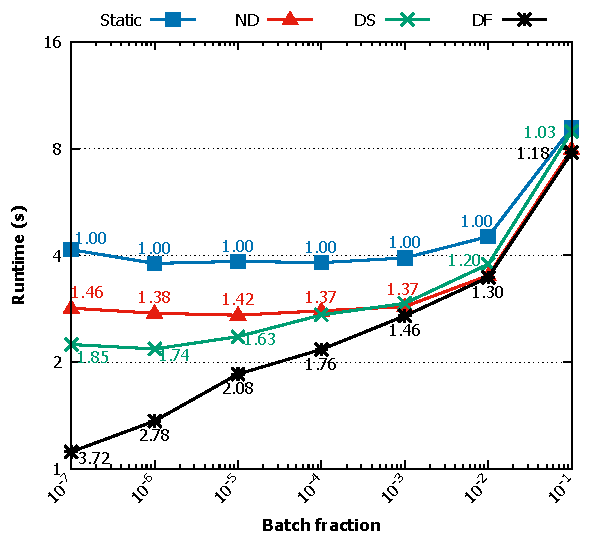
\includegraphics[width=0.38\linewidth]{out/8020-runtime-mean.pdf}
  }
  \subfigure[Results on each graph]{
    \label{fig:8020-runtime--all}
    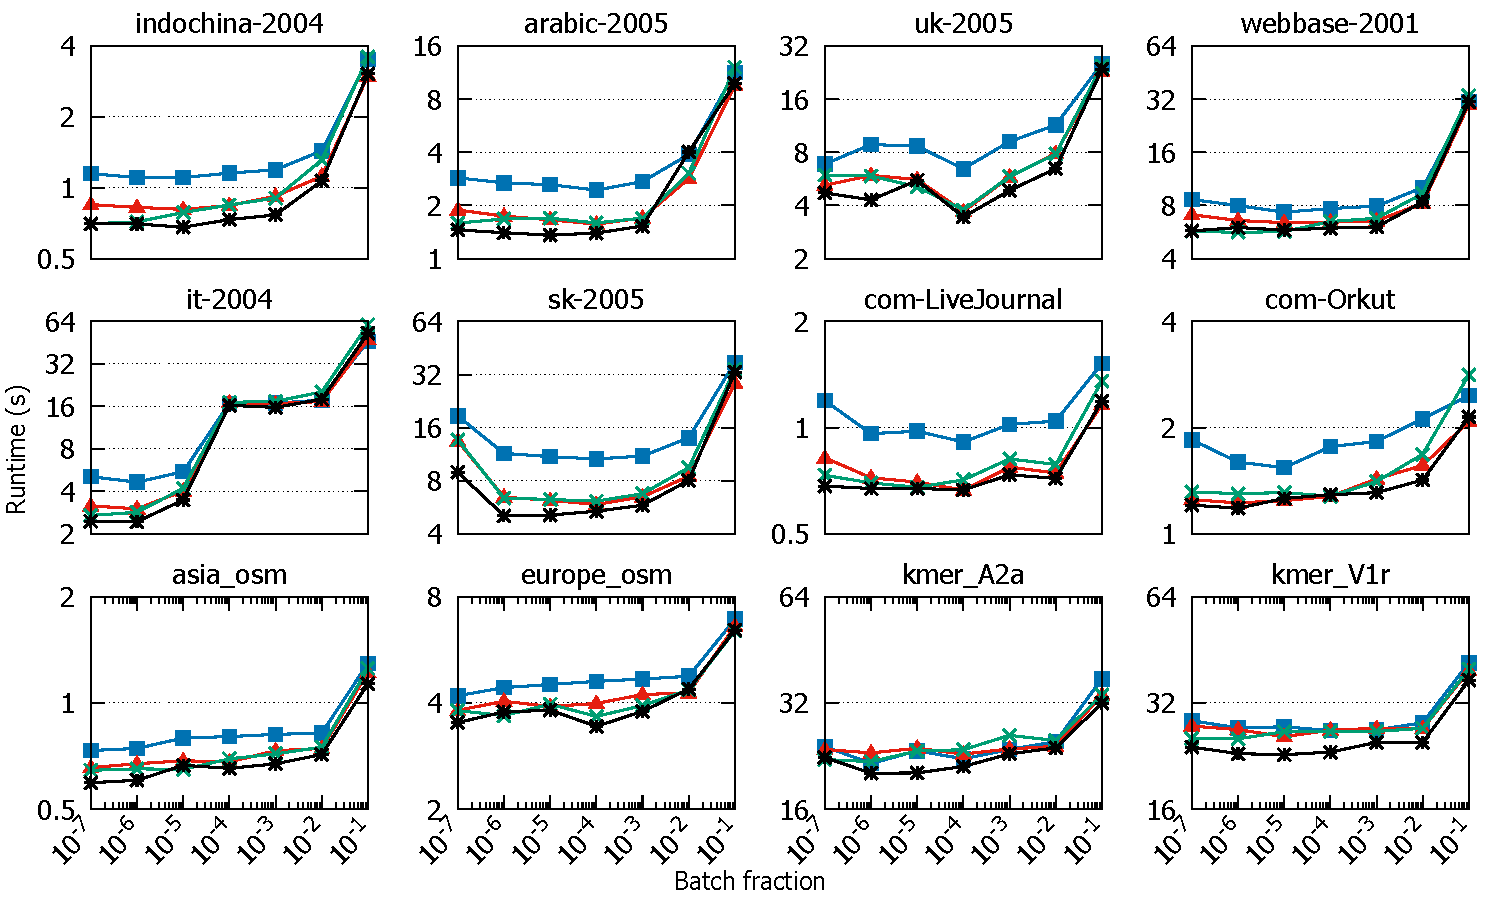
\includegraphics[width=0.58\linewidth]{out/8020-runtime-all.pdf}
  } \\[0ex]
  \caption{Runtime (logarithmic scale) of our multicore implementation of \textit{Naive-dynamic (ND)}, \textit{Delta-screening (DS)}, and \textit{Dynamic Frontier (DF) Leiden}, compared to \textit{Static Leiden} \cite{sahu2024fast}, on large\ignore{(static)} graphs with randomly generated batch updates. The size of these batch updates ranges from $10^{-7}|E|$ to $0.1|E|$ in multiples of $10$, with the updates comprising $80\%$ edge insertions and $20\%$ edge deletions to simulate realistic dynamic graph changes. The right subfigure shows the runtime of each algorithm for individual graphs in the dataset, while the left subfigure displays overall runtimes using the geometric mean for consistent scaling across graphs.\ignore{Furthermore,} The speedup of each algorithm compared to Static Leiden is indicated on the respective lines.}
  \label{fig:8020-runtime}
\end{figure*}

\begin{figure*}[hbtp]
  \centering
  \subfigure[Overall result]{
    \label{fig:8020-modularity--mean}
    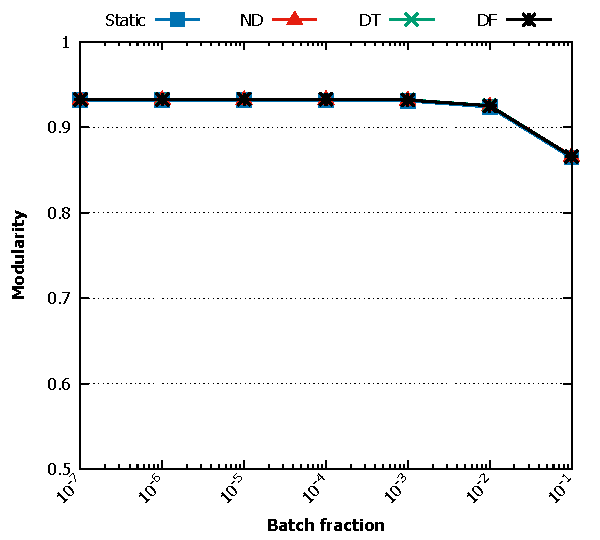
\includegraphics[width=0.38\linewidth]{out/8020-modularity-mean.pdf}
  }
  \subfigure[Results on each graph]{
    \label{fig:8020-modularity--all}
    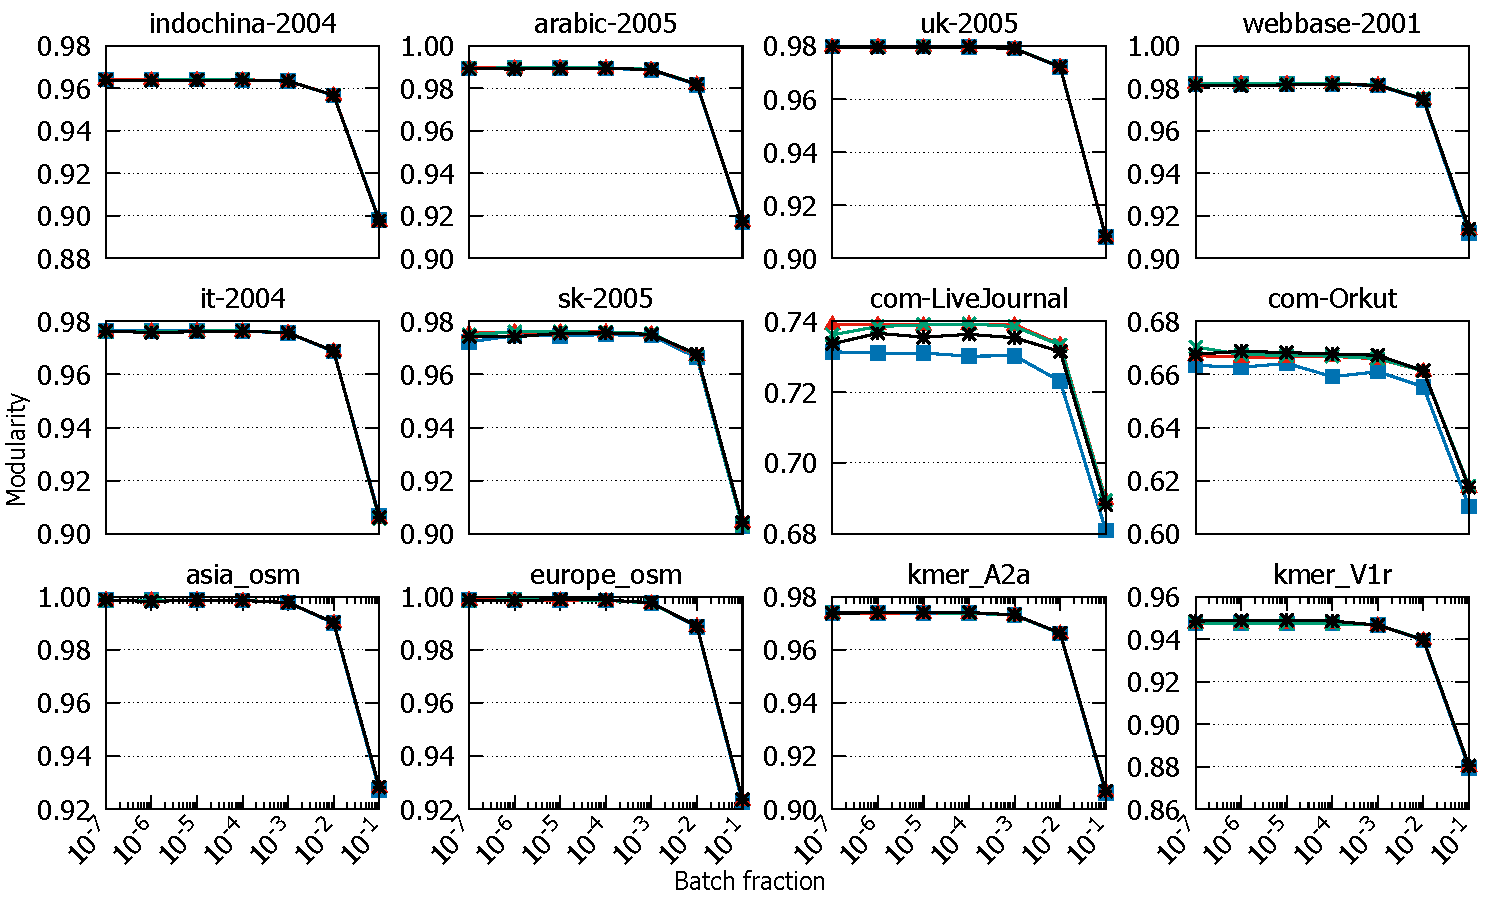
\includegraphics[width=0.58\linewidth]{out/8020-modularity-all.pdf}
  } \\[-2ex]
  \caption{Modularity comparison of our multicore implementation of \textit{Static}, \textit{Naive-dynamic (ND)}, \textit{Delta-screening (DS)}, and \textit{Dynamic Frontier (DF)} Leiden on large (static) graphs with generated random batch updates. The size of batch updates range from $10^{-7} |E|$ to $0.1 |E|$ in multiples of $10$ (logarithmic scale), consisting of $80\%$ edge insertions and $20\%$ edge deletions to simulate realistic dynamic graph updates. The right subfigure depicts the modularity for each approach in relation to each graph, while the left subfigure showcases overall modularity using arithmetic mean.}
  \label{fig:8020-modularity}
\end{figure*}

% \begin{figure*}[!hbt]
  \centering
  \subfigure[Overall Runtime]{
    \label{fig:temporal-summary--runtime-overall}
    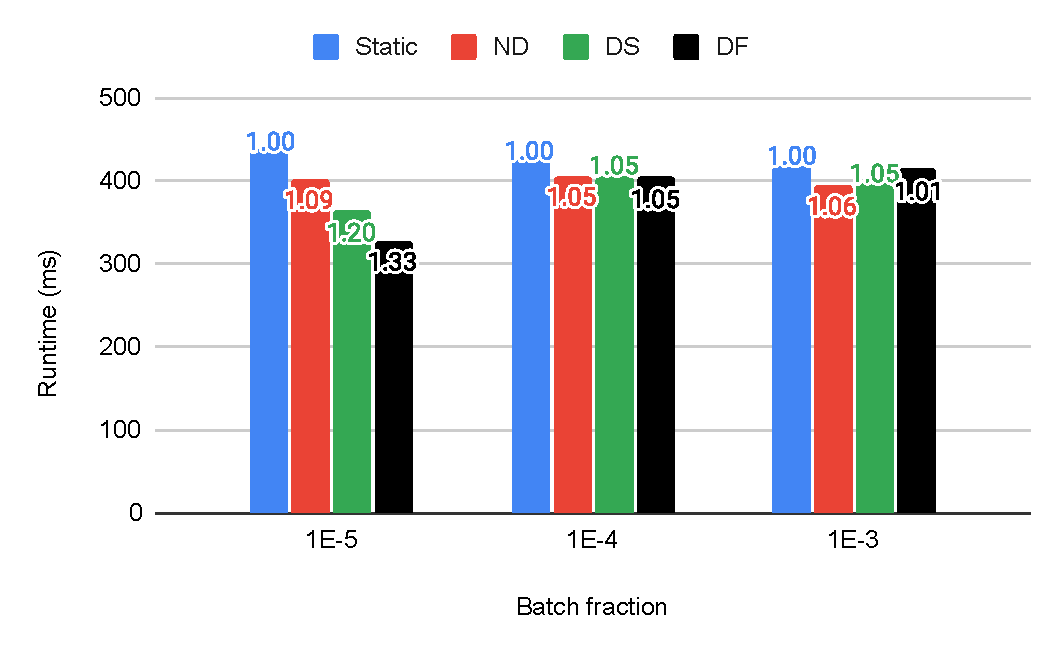
\includegraphics[width=0.48\linewidth]{out/temporal-summary-runtime-overall.pdf}
  }
  \subfigure[Overall Modularity of communities obtained]{
    \label{fig:temporal-summary--modularity-overall}
    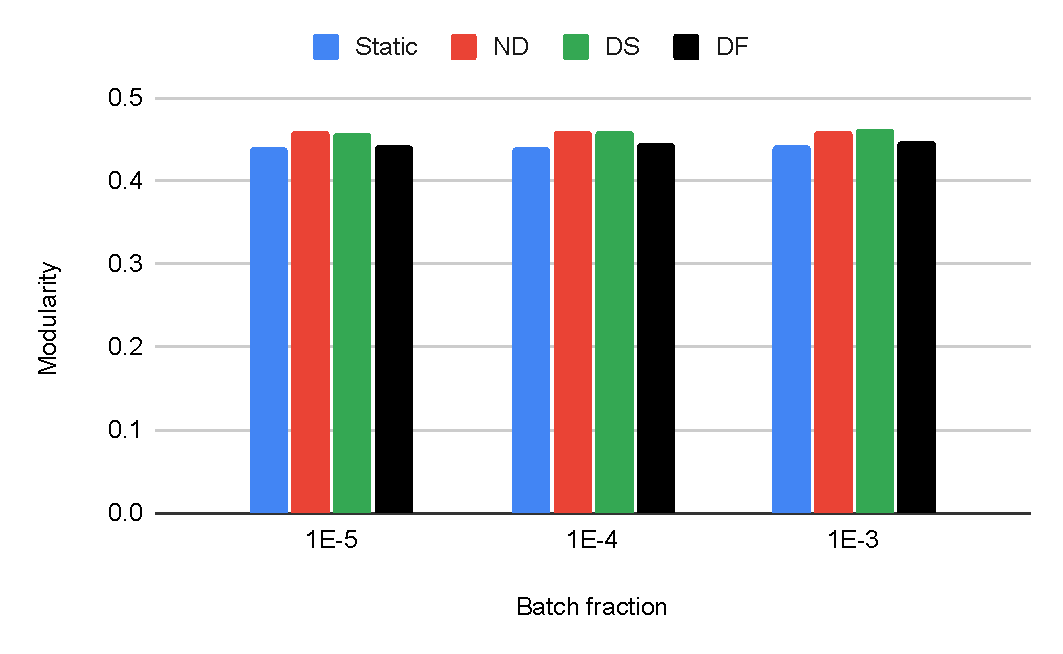
\includegraphics[width=0.48\linewidth]{out/temporal-summary-modularity-overall.pdf}
  } \\[2ex]
  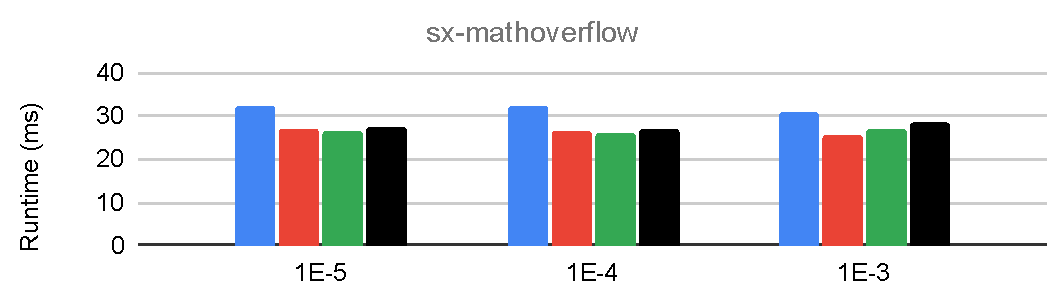
\includegraphics[width=0.48\linewidth]{out/temporal-summary-runtime-sx-mathoverflow.pdf}
  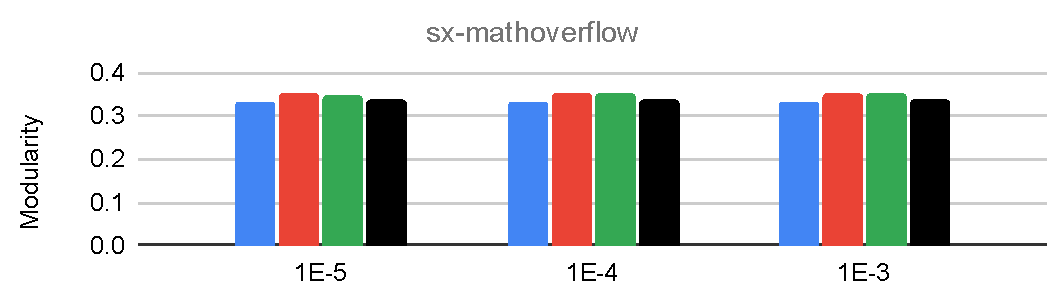
\includegraphics[width=0.48\linewidth]{out/temporal-summary-modularity-sx-mathoverflow.pdf}
  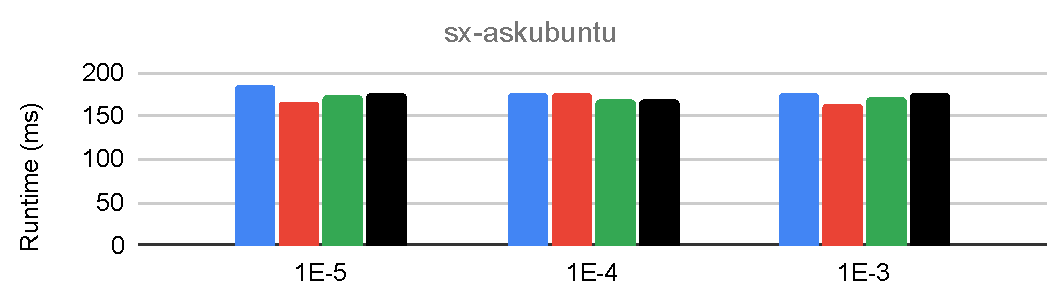
\includegraphics[width=0.48\linewidth]{out/temporal-summary-runtime-sx-askubuntu.pdf}
  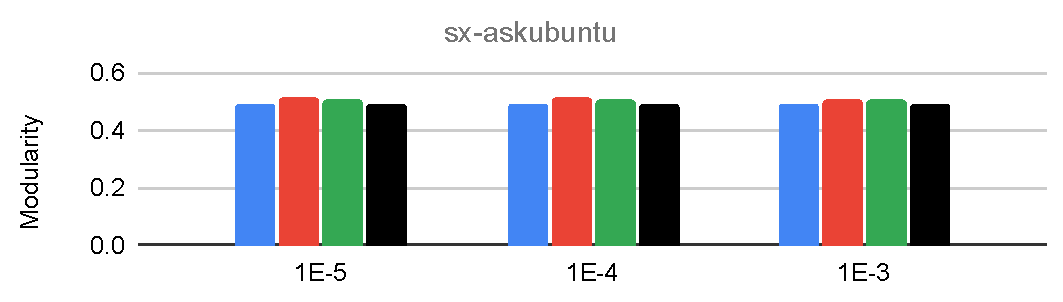
\includegraphics[width=0.48\linewidth]{out/temporal-summary-modularity-sx-askubuntu.pdf}
  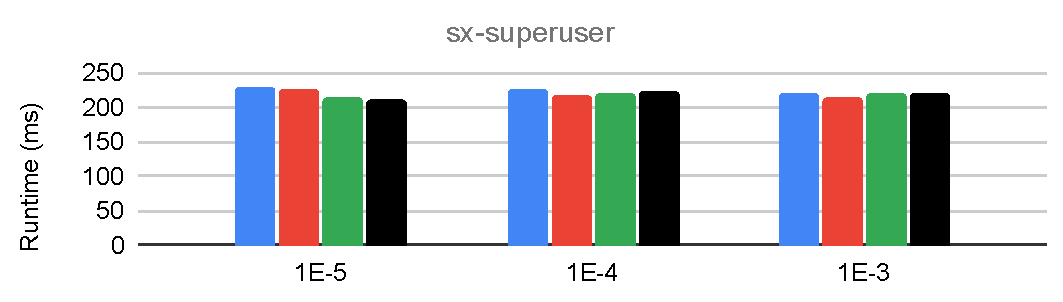
\includegraphics[width=0.48\linewidth]{out/temporal-summary-runtime-sx-superuser.pdf}
  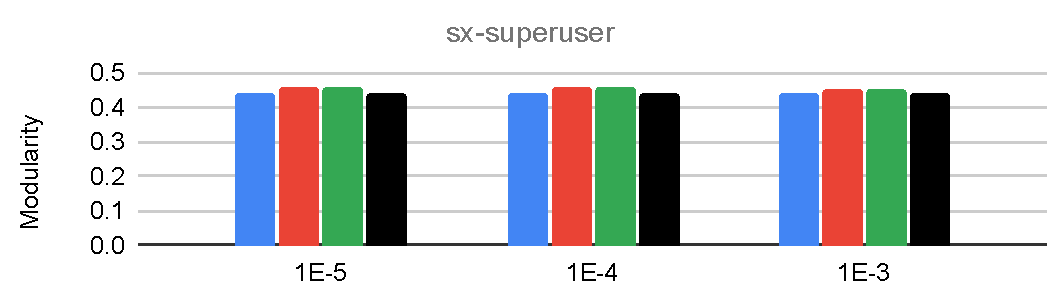
\includegraphics[width=0.48\linewidth]{out/temporal-summary-modularity-sx-superuser.pdf}
  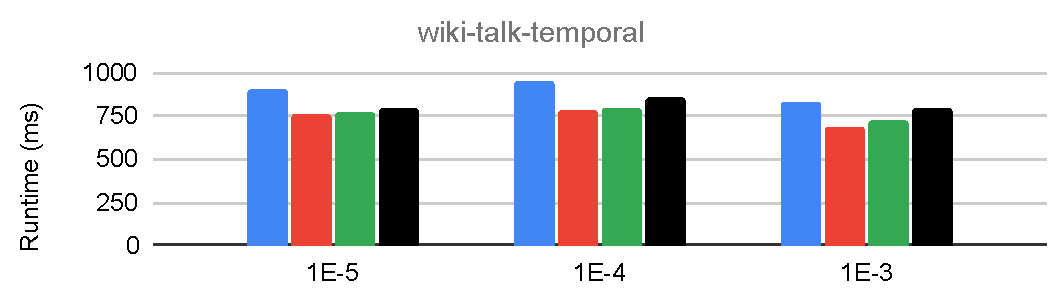
\includegraphics[width=0.48\linewidth]{out/temporal-summary-runtime-wiki-talk-temporal.pdf}
  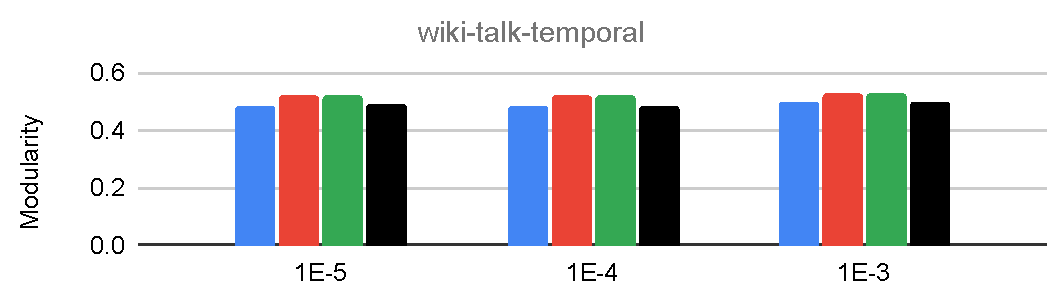
\includegraphics[width=0.48\linewidth]{out/temporal-summary-modularity-wiki-talk-temporal.pdf}
  \subfigure[Runtime on each dynamic graph]{
    \label{fig:temporal-summary--runtime-graph}
    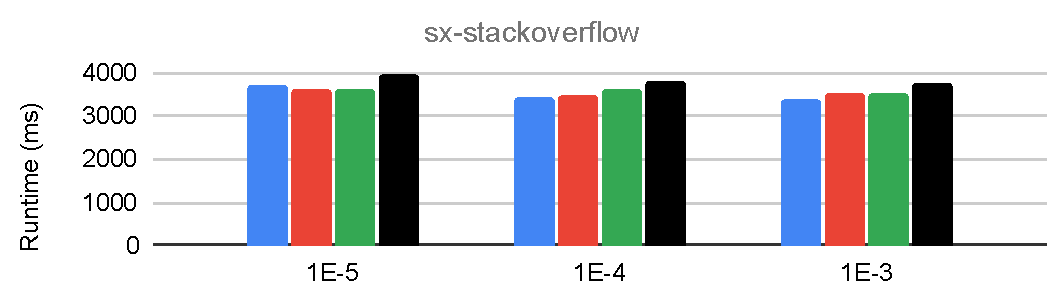
\includegraphics[width=0.48\linewidth]{out/temporal-summary-runtime-sx-stackoverflow.pdf}
  }
  \subfigure[Modularity in communities obtained on each dynamic graph]{
    \label{fig:temporal-summary--modularity-graph}
    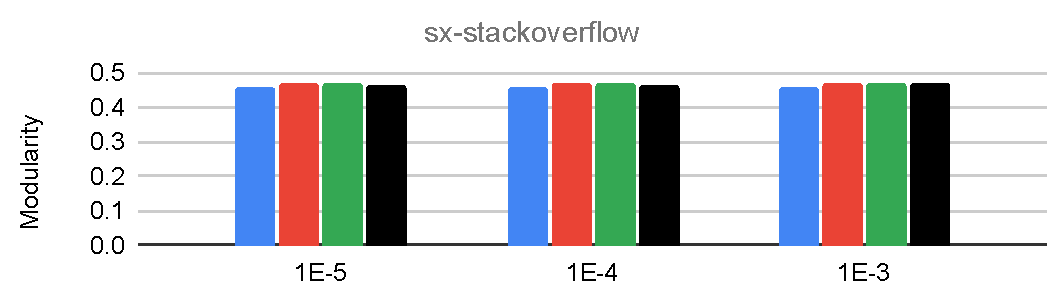
\includegraphics[width=0.48\linewidth]{out/temporal-summary-modularity-sx-stackoverflow.pdf}
  } \\[-2ex]
  \caption{Mean Runtime and Modularity of communities obtained with our multicore implementation of \textit{Static}, \textit{Naive-dynamic (ND)}, \textit{Delta-screening (DS)}, and \textit{Dynamic Frontier (DF)} Leiden on real-world dynamic graphs, with batch updates of size $10^{-5}|E_T|$ to $10^{-3}|E_T|$. Here, (a) and (b) show the overall runtime and modularity across all temporal graphs, while (c) and (d) show the runtime and modularity for each graph. In (a), the speedup of each approach with respect to Static Leiden is labeled.}
  \label{fig:temporal-summary}
\end{figure*}





\subsection{Performance Comparison}
\label{sec:performance-comparison}

We now evaluate the performance of our parallel implementations of ND, DS, and DF Leiden against Static Leiden \cite{sahu2024fast}, on large graphs with randomly generated batch updates. Static Leiden is rerun from scratch after each update, whereas ND, DS, and DF Leiden begin with prior community assignments. Additionally, DS and DF Leiden identify affected vertices, processing only these during local-moving phase. Our methods are applicable to ND, DS, and DF Leiden. Original Leiden \cite{com-traag19} is sequential; thus we compare against the fastest parallel Leiden \cite{sahu2024fast}. As detailed in Section \ref{sec:batch-generation}, these updates range in size from $10^{-7}|E|$ to $0.1|E|$, with $80\%$ edge insertions and $20\%$ edge deletions. Each batch update includes reverse edges to keep the graph undirected. Figure \ref{fig:8020-runtime--all} presents the execution time of each algorithm across individual graphs, while Figure \ref{fig:8020-runtime--mean} depicts overall runtimes using geometric mean for consistent scaling across differing graph sizes. In addition, Figure \ref{fig:8020-modularity--all} shows the modularity of the algorithms for individual graphs in the dataset, and Figure \ref{fig:8020-runtime--mean} presents the overall modularity of each of the algorithms, calculated using arithmetic mean.

From Figure \ref{fig:8020-runtime--mean}, we observe that ND, DS, and DF Leiden achieve mean speedups of $1.37\times$, $1.47\times$, and $1.98\times$, respectively, when compared to Static Leiden. This speedup is higher on smaller batch updates, with ND, DS, and DF Leiden being on average $1.46\times$, $1.74\times$, and $3.72\times$, respectively, when compared to Static Leiden, on batch updates of size $10^{-7}|E|$. Figure \ref{fig:8020-runtime--all} shows that ND, DS, and DF Leiden offer moderate speedups over Static Leiden on web graphs and social networks --- while on road networks (with low average degree), ND Leiden marginally outperforms Static Leiden, and DS and DF Leiden perform significantly better. This is due to DS and DF Leiden processing significantly fewer affected vertices/communities on road networks. On protein k-mer graphs, DS Leiden offers only a slight improvement. However, on small batch updates, DF Leiden outperforms Static Leiden by a large margin.

In terms of modularity, as Figures \ref{fig:8020-modularity--mean} and \ref{fig:8020-modularity--all} show, ND, DS, and DF Leiden achieve communities with approximately the same modularity as Static Leiden. However, on social networks, ND, DS, and DF Leiden moderately outperform Static Leiden. This is likely due to social networks not having a strong enough community structure, and thus requiring more iterations to converge to a better community assignment. On such graphs, Static Leiden fails to attain better modularity due to it limiting the number of iterations per pass performed, in favor of faster runtimes. However, since ND, DS, and DF Leiden do not start from scratch, but leverage prior community assignments, they are able to converge faster, and with higher modularity than Static Leiden (Figure \ref{fig:8020-modularity}) --- particularly on social networks, where poor community structures make clustering more challenging. Thus, on average, the modularity of communities from Static Leiden is slightly lower. However, we notice that modularity of communities identified by our algorithms do not differ by more than $0.002$ from Static Leiden, on average.

Also note in Figure \ref{fig:8020-runtime} that the runtime of Static Leiden increases with larger batch updates. This effect is primarily due to two factors: \textbf{(1)} Larger batches increase graph size, as $80\%$ of updates are edge insertions; and \textbf{(2)} Random edge updates disrupt original community structure, requiring more iterations to converge. This\ignore{disruption} also accounts for the observed decline in modularity of the algorithms with larger batch sizes, as seen in Figure \ref{fig:8020-modularity}.

Let us now discuss why ND, DS, and DF Leiden exhibit only modest speedups over Static Leiden. Unlike Louvain algorithm, we must always run the refinement phase of Leiden algorithm to avoid badly connected and internally disconnected communities. Nonetheless, the refinement phase splits the communities obtained/updated from the local-moving phase into several smaller sub-communities. Stopping the passes early\ignore{, as done with DF Louvain,} leads to low modularity scores for ND/DS/DF Leiden because sufficiently large high-quality clusters have not yet formed\ignore{due to the refinement phase}. Further, ND/DS/DF Leiden can only reduce the runtime of the local-moving phase of the first pass of the Leiden algorithm. However, only about $37\%$ of the runtime in Static Leiden is spent in the local-moving phase of the first pass. These factors constrain the speedup potential of ND, DS, and DF Leiden over Static Leiden. Regardless, on large graphs with random batch updates, DF Leiden appears to be the dynamic community detection method of choice for tracking evolving communities. Performance comparison on real-world dynamic graphs is given in Section \ref{sec:performance-comparison-temporal}.




\subsection{\ignore{Analysis of }Affected vertices and Changed communities}

We now study the fraction of vertices marked as affected, and the communities marked as changed (to keeping track of the subset of communities to be refined), by DS and DF Leiden on instances from Table \ref{tab:dataset-large}, with batch updates ranging from $10^-7|E|$ to $0.1|E|$. This tracking occurs only in the first pass of the Leiden algorithm, as detailed in Sections \ref{sec:subset-refine-method} and \ref{sec:optimized-aggregation-method}, and is shown in Figure \ref{fig:8020-affected}.
% We now study the fraction of vertices marked as affected, and the fraction of communities marked as changed (used for keeping track of the subset of communities to be refined), by DS and DF Leiden. We do this over the instances in Table \ref{tab:dataset-large}, on batch updates of size $10^-7|E|$ to $0.1|E|$. Note that we only keep track of affected vertices and changed communities in the first pass of Leiden algorithm, as mentioned in Sections \ref{sec:subset-refine-method} and \ref{sec:optimized-aggregation-method}, and this is what is measure in Figure \ref{fig:8020-affected}.

\begin{figure}[hbtp]
  \centering
  \subfigure{
    \label{fig:8020-affected--all}
    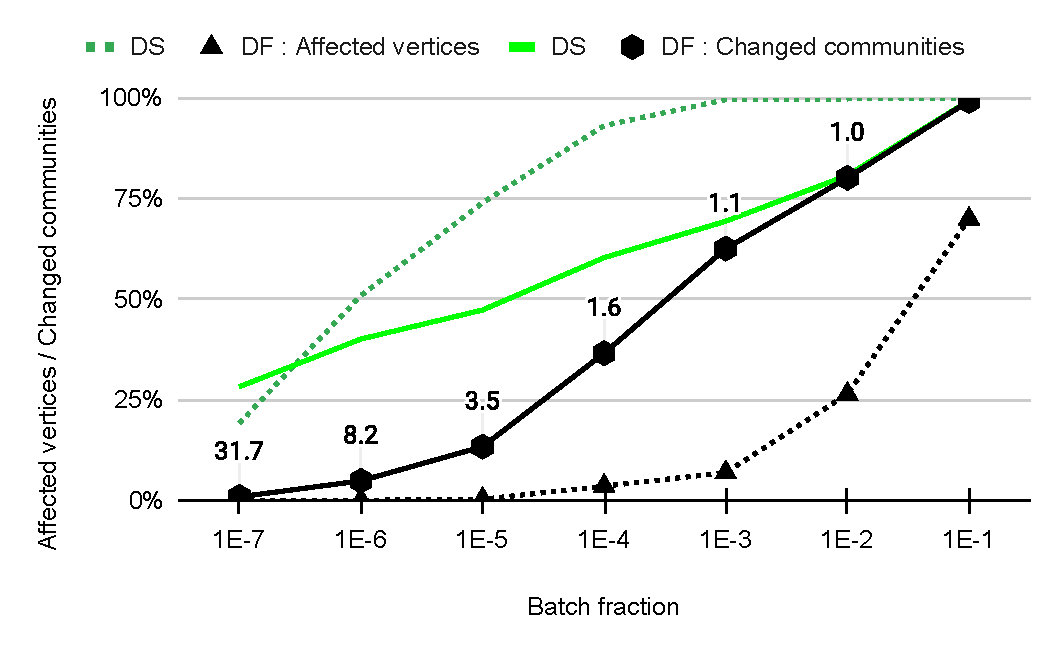
\includegraphics[width=0.98\linewidth]{out/8020-affected.pdf}
  } \\[-4ex]
  \caption{Fraction of vertices marked as affected (dotted lines), and communities marked as changed (solid lines) with \textit{Delta-screening (DS)} and \textit{Dynamic Frontier (DF) Leiden} on graphs in Table \ref{tab:dataset-large}. The labels indicate the ratio of communities marked as changed by DS Leiden to that of DF Leiden.}
  \label{fig:8020-affected}
\end{figure}

\begin{figure}[hbtp]
  \centering
  \subfigure{
    \label{fig:8020-scaling--am}
    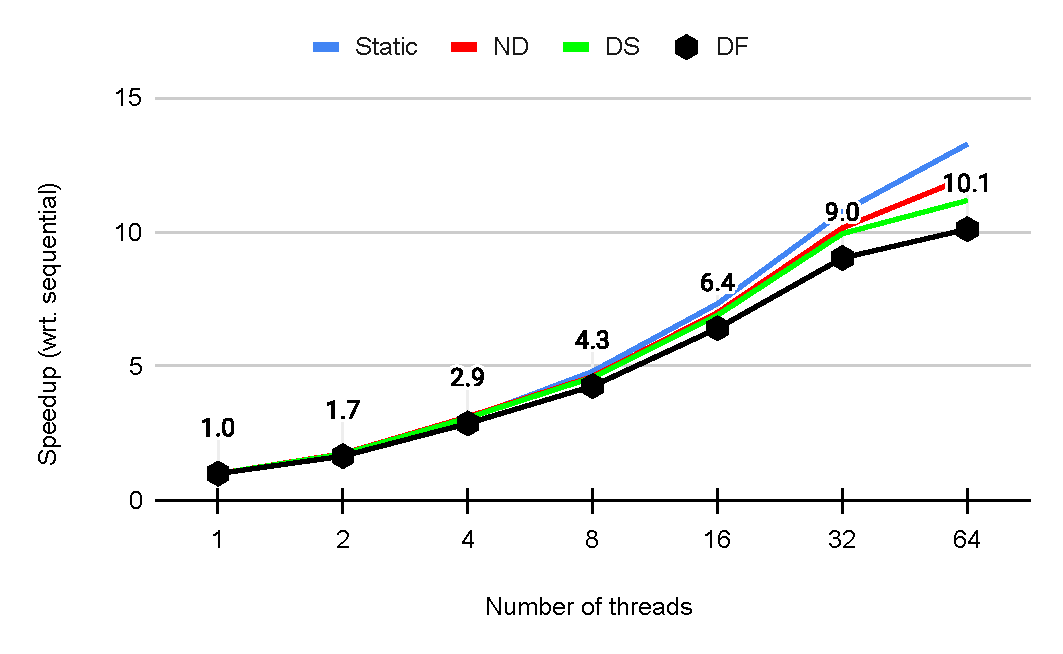
\includegraphics[width=0.98\linewidth]{out/8020-scaling.pdf}
  } \\[-1ex]
  \caption{Strong scalability of ND, DS, and DF Leiden on batch updates of size $10^{-3} |E|$. The number of threads is doubled from $1$ to $64$ (logarithmic scale) \su{TO BE UPDATED}.}
  \label{fig:8020-scaling}
\end{figure}


We notice from Figure \ref{fig:8020-affected} that DF Leiden marks fewer affected vertices and changed communities than DS Leiden, but their runtime difference is smaller, as many vertices marked by DS Leiden do not change their community labels, and converge quickly. However, as expected, performance of the algorithms decline with more affected vertices, as Figures \ref{fig:8020-runtime} and \ref{fig:8020-affected} show. Further, while a high number of changed communities increases refinement costs in the first pass, the cost of subsequent passes\ignore{is more or less constant, and} only depends on the graph's nature.
% We notice from Figure \ref{fig:8020-affected} that DF Leiden marks a significantly smaller fraction of vertices as affected and a decently smaller fraction of communities as changed, compared to DS Leiden. The runtime of these algorithms, however, do not differ in this ratio as DS Leiden marks entire communities of vertices as affected but many such affected vertices may not really undergo a change in their community label. So, a large fraction of such affected vertices converge in only one iteration.  Also, as Figures \ref{fig:8020-runtime} and \ref{fig:8020-affected} show, the performance of our algorithms drops as more vertices are marked as affected. In addition, while, a large number of changed communities tend to proportionally increase the cost of refinement phase in the first pass of the algorithm, the cost of the remaining passes is more of less constant, and only depends on the nature of the updated graph.




\subsection{Scalability}

Finally, we study the strong-scaling behavior of ND, DS, and DF Leiden, and compare it with Static Leiden. For this, we fix the batch size at $10^{-3} |E|$, vary the\ignore{number of} threads\ignore{in use} from $1$ to $64$, and measure the speedup of each algorithm with respect to its sequential version.

As shown in Figure \ref{fig:8020-scaling}, ND, DS, and DF Leiden obtain a speedup of $10.2\times$, $9.9\times$, and $9.0\times$ respectively at $32$ threads (with respect to sequential\ignore{execution}); with their speedup increasing at a mean rate of $1.59\times$, $1.58\times$, and $1.55\times$, respectively, for every doubling of threads. At $64$ threads, NUMA affects the performance of our algorithms (NPS 4). In addition, increasing the number of threads makes the behavior of the algorithm less asynchronous, i.e., similar to the Jacobi iterative method, further contributing to the performance drop.




% \su{Finding densest community}
% If quality corresponds to modularity, one can pick the community with the largest modularity score to be the one of highest quality (densest subgraph).




% \subsection{Stability of communities identified}

% Intuitively, if the graphs $G^t$ and $G^{t'}$ are identical for some $t$ and $t'$, we expect DF Leiden to produce the same communities for $G^t$ and $G^{t'}$. We refer to this property of a dynamic algorithm as its stability, measured as the percentage of vertices that agree on the community label across two identical graphs. Vertices within weak community structures tend to be unstable, as they may connect to multiple communities with similar strength.

% To measure the stability of DF Leiden, we proceed as follows. Let $G$ be an initial graph. We generate a batch update of size $10^{-7} |E|$ to $0.1 |E|$ consisting of edge deletions to obtain the graph $G^1$. We then apply each of the above algorithms on $G^1$ to identify the new communities. Subsequently, we create another batch of updates that inserts the edges deleted in the prior time step. This graph, $G^2$, is essentially the original graph $G$. We obtain the community labels of the vertices in the graph $G^2$ by appealing to the dynamic algorithms. Finally, we compare the community label of each vertex in the graphs $G$ and $G^2$. We observe that DF Leiden has a minimum of $99.70\%$ match, thus indicating that it is stable.

% In strong community structures, vertices tend to be stable and well-connected within their community. Weak community structures can result in unstable vertices, as they may connect to multiple communities with similar strength.




% \subsection{Further discussion}

% \subsubsection{Results on real-world dynamic graphs}

% We also evaluate the performance of our parallel implementations of Static, ND, DS, and DF Leiden on real-world dynamic graphs listed in Table \ref{tab:dataset}. These evaluations are performed on batch updates ranging from $10^{-5}|E_T|$ to $10^{-3}|E_T|$ in multiples of $10$. For each batch size, as described in Section \ref{sec:batch-generation}, we load $90\%$ of the graph, add reverse edges to ensure all edges are undirected, and then load $B$ edges (where $B$ is the batch size) consecutively in $100$ batch updates. Figure \ref{fig:temporal-summary--runtime-overall} shows the overall runtime of each approach across all graphs for each batch size, while Figure \ref{fig:temporal-summary--modularity-overall} depicts the overall modularity of the obtained communities. Additionally, Figures \ref{fig:temporal-summary--runtime-graph} and \ref{fig:temporal-summary--modularity-graph} present the mean runtime and modularity of the communities obtained with each approach on individual dynamic graphs in the dataset.

% Figure \ref{fig:temporal-summary--runtime-overall} illustrates that ND Leiden is, on average, $1.09\times$ faster than Static Leiden for batch updates ranging from $10^{-5}|E_T|$ to $10^{-3}|E_T|$. In comparison, DS and DF Leiden exhibit average speedups of $1.20\times$ and $1.33\times$, respectively, over Static Leiden for the same batch updates. We now explain why ND, DS, and DF Leiden achieve only minor speedups over Static Leiden. Our experiments indicate that only about $20\%$ of the overall runtime of Static Leiden is spent in the local-moving phase of the first pass.\ignore{This is a significant decrease from the $37\%$ observed on large graphs with random batch updates.} Consequently, the speedup achieved by ND, DS, and DF Leiden relative to Static Leiden is limited. Furthermore, our observations suggest that while DF Leiden can reduce the time spent in the local-moving phase slightly more than ND Leiden, it incurs increased runtimes in the refinement and aggregation phases of the algorithm. This is likely because ND Leiden is able to optimize clusters more effectively than DF Leiden, which accelerates the refinement and aggregation phases for ND Leiden, albeit by a small margin. This explains the lower speedup of DF Leiden compared to ND Leiden on larger batch updates\ignore{of real-world dynamic graphs}.\ignore{Therefore, we recommend ND Leiden for real-world dynamic graphs.}

% Unlike with large graphs and random batch updates, on real-world dynamic graphs, we disable the aggregation tolerance $\tau_{agg}$. This results in a reduced portion of runtime spent in the local-moving phase of the first pass, which is the phase that can be minimized by the dynamic approaches. Specifically, we observe that only about $20\%$ of the overall runtime of Static Leiden is spent in the local-moving phase of the first pass.
